\documentclass[11pt]{article}
\usepackage{url,graphicx,tabularx,array,amsmath,amssymb,amsthm,booktabs,float}
\usepackage[margin=.65in]{geometry}
\graphicspath{C:/Users/Colin/Documents/GitHub/SMOS/simulation}
\setlength{\parskip}{1ex} %--skip lines between paragraphs
\setlength{\parindent}{0pt} %--don't indent paragraphs


\DeclareGraphicsRule{.tif}{png}{.png}{`convert #1 `dirname #1`/`basename #1 .tif`.png}
\newcommand{\vcentergraphics}[2]{\ensuremath{\vcenter{\hbox{\includegraphics[#1]{#2}}}}}


%-- Commands for header
\renewcommand{\title}[1]{\textbf{#1}\\}
\renewcommand{\line}{\begin{tabularx}{\textwidth}{X>{\raggedleft}X}\hline\\\end{tabularx}\\[-0.5cm]}
\newcommand{\leftright}[2]{\begin{tabularx}{\textwidth}{X>{\raggedleft}X}#1%
& #2\\\end{tabularx}\\[-0.5cm]}


\begin{document}


\title{Pixel 194406}
\line
\leftright{9.2.16}{Colin Lewis-Beck} %-- left and right positions in the header

\begin{description}
\item \textit{2 Harmonics:}\\
Let's fit a constant DLM with the following specification:

\begin{equation*}
\begin{align}
Y_t&=F\theta_t+v_t &\ v_t \sim N(0,\sigma^2_o) \\
\theta_t&=G\theta_{t-1}+w_t &\ w_t \sim N(0,\sigma^2_e)\\
S_{jt}&=\text{cos}(t\omega_j)S_{j,t-1}+\text{sin}(t\omega_j)S^*_{j,t-1}\\
S^*_{jt}&=-\text{sin}(t\omega_j)S_{j,t-1}+\text{cos}(t\omega_j)S^*_{j,t-1}\\
\end{align}
\end{equation}
\text{where,}
\begin{equation*}
\begin{align}
\theta_t&=[S_{1t},S^*_{1t},S_{2t},S^*_{2t}], &\  F=[1,0,1,0] \\
 \omega_j&=\frac{2 \pi j}{s}, j=1,2, s=276
\end{align}
\end{equation}
\begin{align*}
G = \begin{bmatrix}
\text{cos}(\omega_1) & \text{sin}(\omega_1) & 0 & 0\\
\text{-sin}(\omega_1) & \text{cos}(\omega_1) & 0 & 0\\
0 & 0 & \text{cos}(\omega_2) & \text{sin}(\omega_2)\\
0 & 0 & \text{-sin}(\omega_2) & \text{cos}(\omega_2)
\end{bmatrix}
\end{align}
and,
\begin{align*}
W = \begin{bmatrix}
\sigma^2_e & 0 & 0 & 0\\
0 & \sigma^2_e & 0 & 0\\
0 & 0 & \sigma^2_e & 0\\
0 & 0 & 0 & \sigma^2_e
\end{bmatrix}
\end{align}
We have 5 years of data so, $t=1 \dots T=1650$ or $T=1656$ depending on the pixel.  To draw from the posterior distribution of $\pi(\theta_{0:t},\sigma_o,\sigma_e|y_{1:t})$ we use a Gibbs sampler with an IG prior on the variance parameters, which is a conjugate prior when combined with the normality assumption on the observed and state space distributions.  Parameterizing in terms of $1/V$ and $W^{-1}$, we have $1/\sigma_o\sim \mathcal{G}(a_1=1,b_1=1)$ and $1/\sigma_e \sim \mathcal{G}(a_2=1,b_2=1)$.  Starting values for both $1/V$ and $W^{-1}$ were 1. The prior on the state space equation, $N(\underline{\bold{0}},1e^{07}\underline{\bold{1}}}) \\

The posteriors for the parameters are as follows:
\begin{equation*}
\begin{align}
\theta^{(i)}_{0:T} &\sim \pi(\theta_{0:T}|y_{1:T},1/\sigma^{(i-1)}_{o},1/\sigma^{(i-1)}_{e})\\
1/\sigma_{o} &\sim \mathcal{G}\left(a_1+T^{*}/2, b_1+ 1/2 \sum_{t=1}^{T^{*}}(y_t-F\theta_t)^{'}(y_t-F\theta_t)\right)\\
1/\sigma_{e} &\sim \mathcal{G}\left(a_2+2T, b_2+ 1/2 \sum_{t=1}^{T}(\theta_t-G\theta_{t-1})^{'}(\theta_t-G\theta_{t-1})\right)
\end{align}
\end{equation}
Each pixel has missing values, so $T^{*}$ represents the number of non-missing values of $y_t$.
 



\item \textit{Simulation}\\
Let's explore the effect of changing the evolution variance, $W$, on simulated values from a 2 and 3 harmonic DLM model.  In both cases we assume $\theta_0 \sim N_p(m_0,C_0)$.  Depending on the dimension, $m_0={0}$ and ${C_0}=\mathbb{{I}}$.  For both the 2 and 3 harmonic DLMs, we will fix $V=1$.  For each simulation, $s=276$ and $n=1656$.  We will vary the diagonal of the $W$ matrix, which controls the variance of the evolution parameters.  


\begin{figure}[H]
\caption{Simulated 2 Harmonic}
\centering
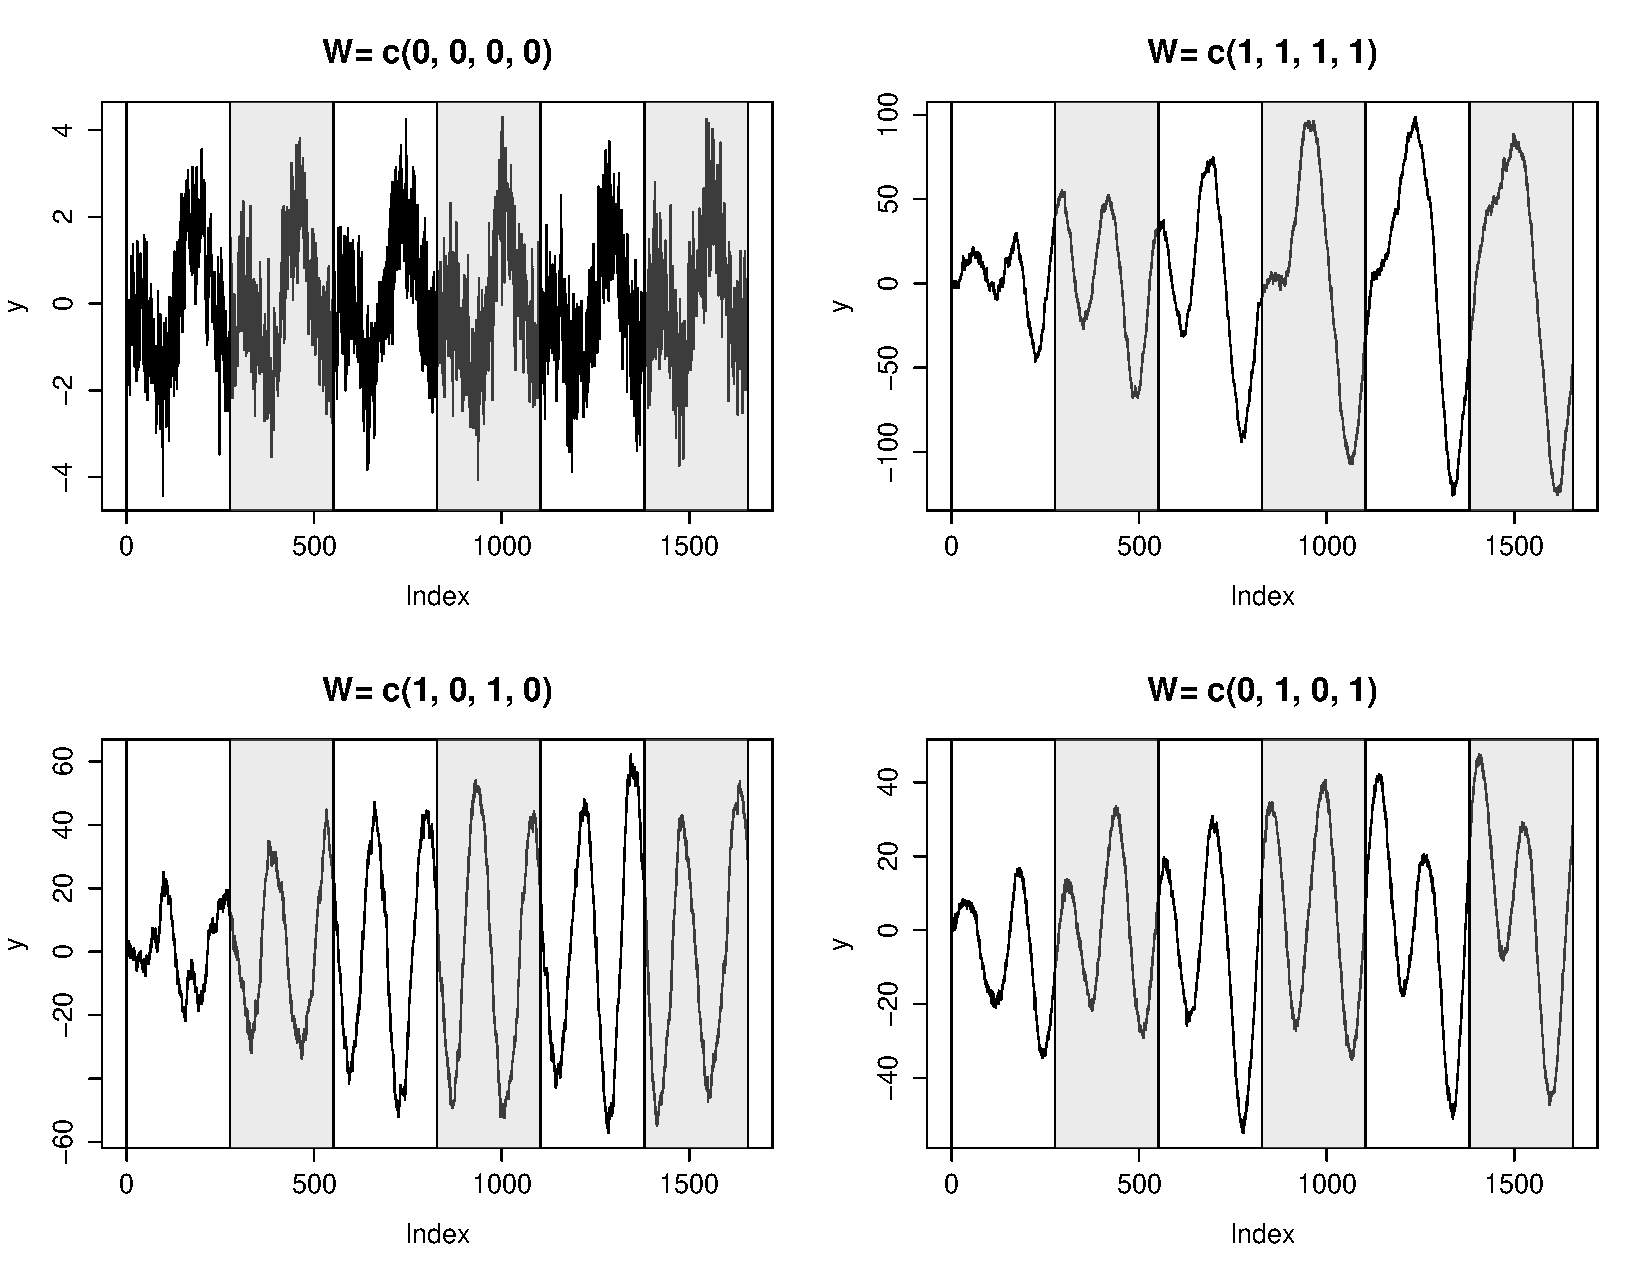
\includegraphics[height=8cm]{harm2_1.pdf}
\end{figure}

\begin{figure}[H]
\caption{Simulated 2 Harmonic}
\centering
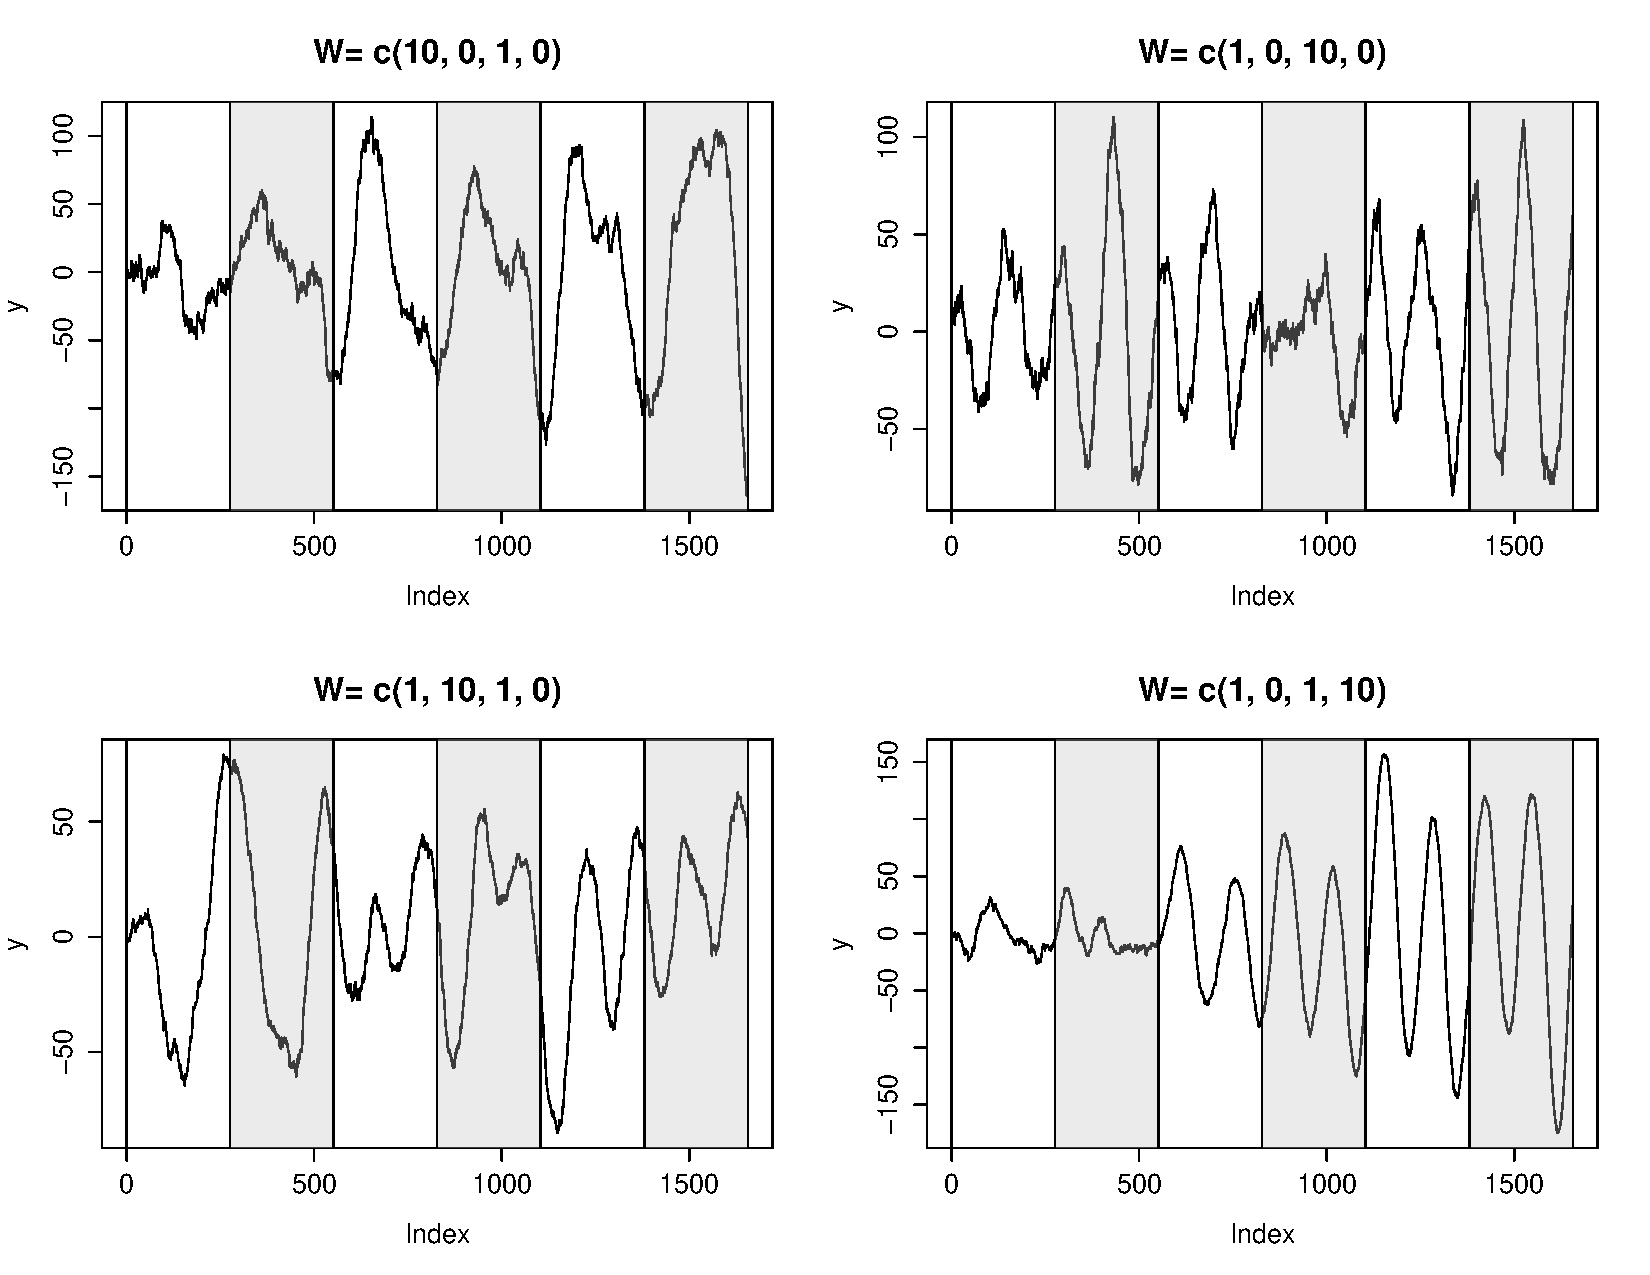
\includegraphics[height=8cm]{harm2_2.pdf}
\end{figure}

\begin{figure}[H]
\caption{Simulated 3 Harmonic}
\centering
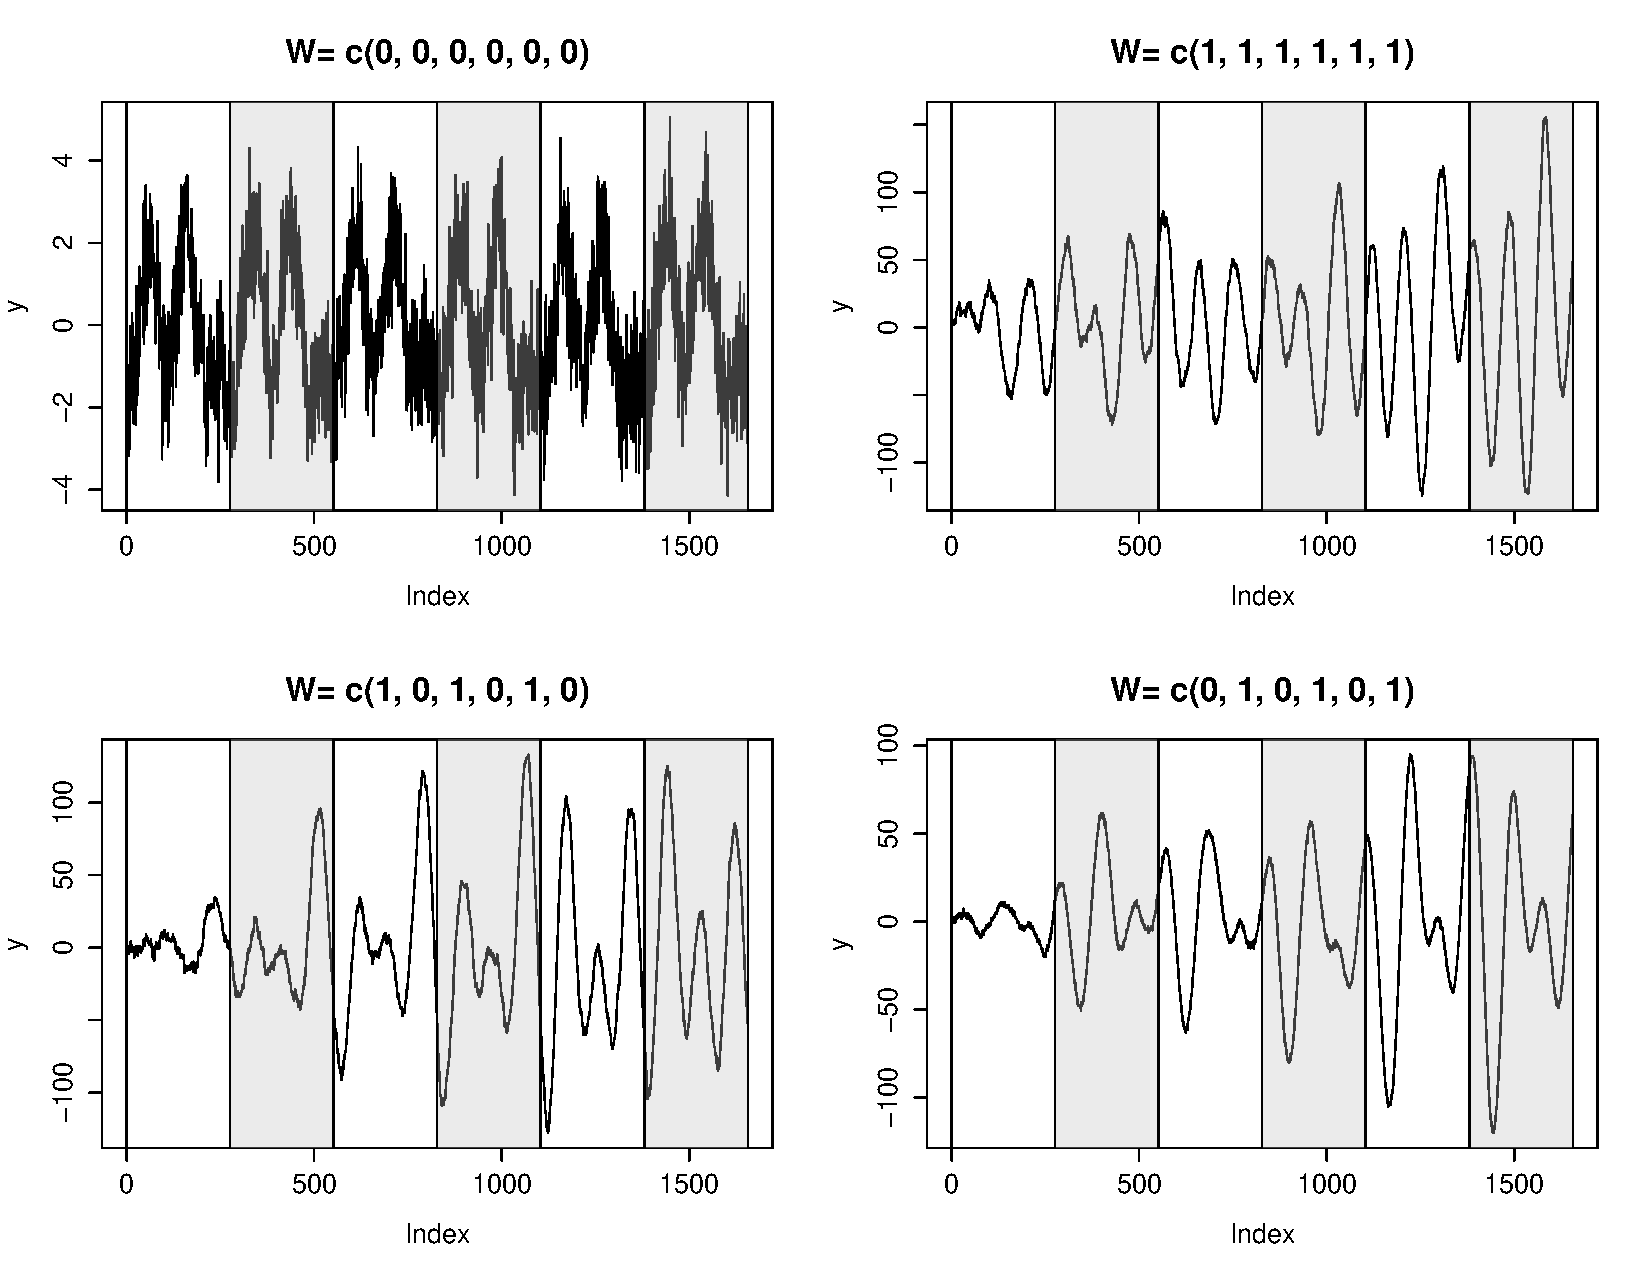
\includegraphics[height=8cm]{harm3_1.pdf}
\end{figure}

\begin{figure}[H]
\caption{Simulated 3 Harmonic}
\centering
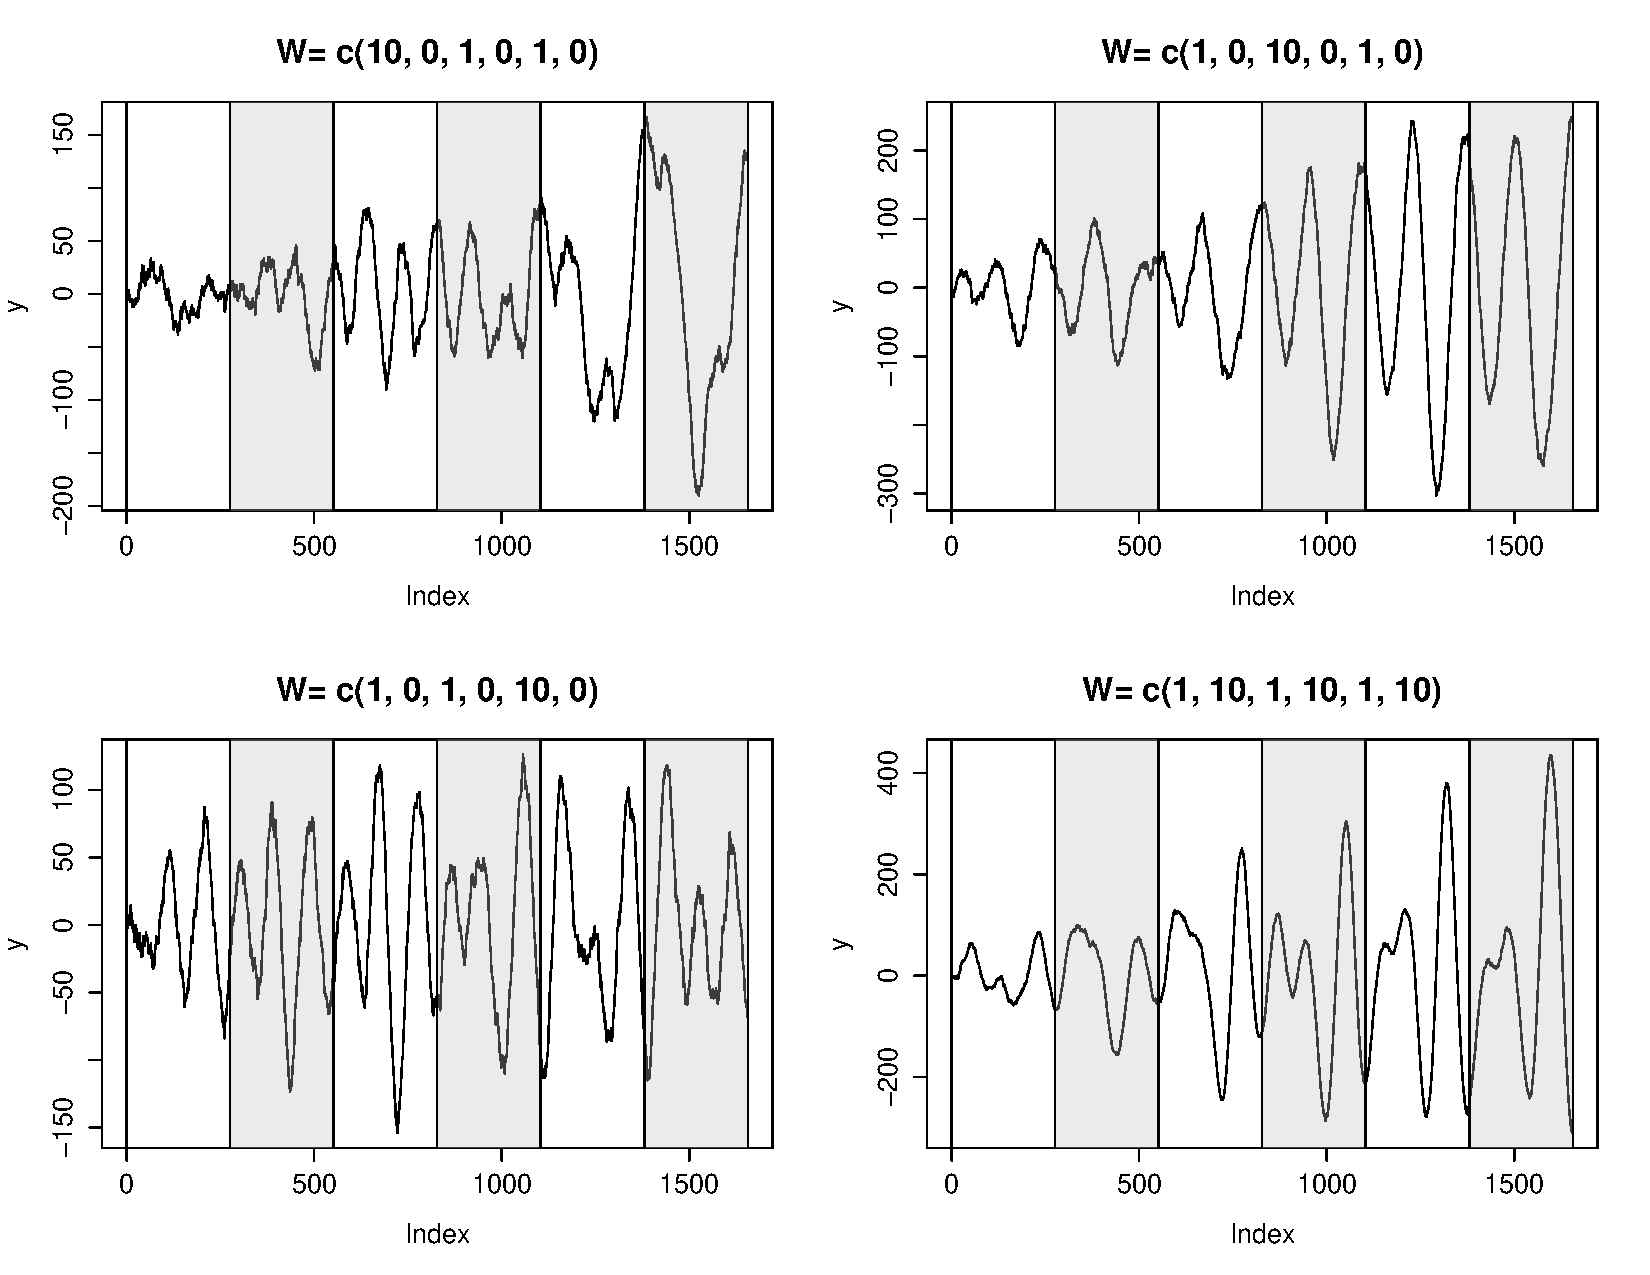
\includegraphics[height=8cm]{harm3_2.pdf}
\end{figure}


The correlation between V and W is fairly small, $\rho$ was between .12 and .16 for all chains.
\newpage
Below is the median of the states plotted above the raw data.
\begin{figure}[H]
\caption{2 Harmonic Regression for Pixel 194406}
\centering
\includegraphics[height=12cm]{pix1_post.pdf}
\end{figure}

\begin{figure}[H]
\caption{MLE Smooth States Pix 194406}
\centering
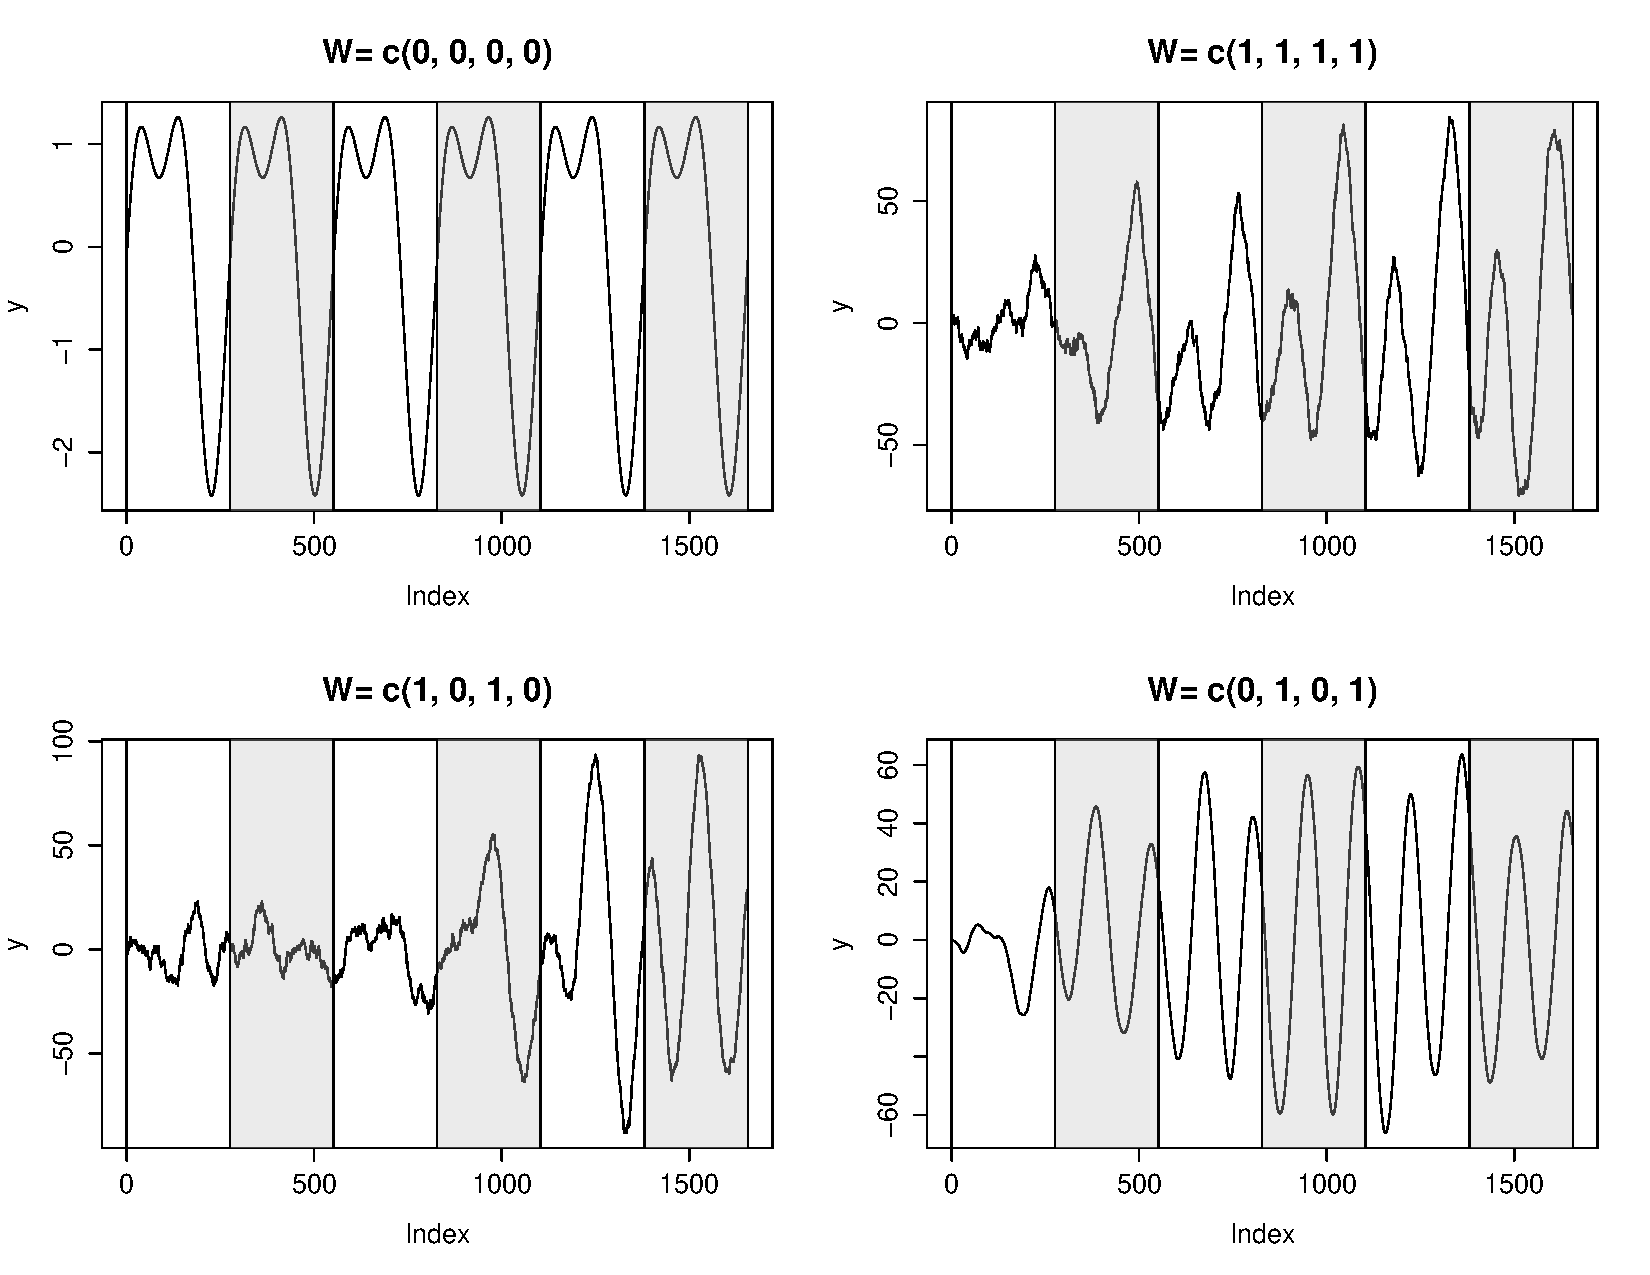
\includegraphics[height=15cm]{harmsim1_zeroV.pdf}
\end{figure}
\newpage

For Pix 203632.  Visually, this location seems to have the least noise of the 30 pixels. 

\begin{figure}[H]
\caption{2 Harmonic Regression for Pixel 203632}
\centering
\includegraphics[height=12cm]{pix30_comp.pdf}
\end{figure}

\begin{figure}[H]
\caption{MLE Smooth States Pix 203632}
\centering
\includegraphics[height=15cm]{pix30_smooth.pdf}
\end{figure}
\newpage

\end{document}